\documentclass{article}
\usepackage[utf8]{inputenc}
\usepackage[margin=1in,includefoot]{geometry}
\usepackage{graphicx}
\usepackage{subcaption}
\usepackage{enumerate}
\usepackage{xfrac}
\usepackage{url}
\usepackage{amsmath}
\usepackage{mathtools}
\usepackage{blindtext}
\usepackage[numbers,sort&compress]{natbib}
\usepackage{listings}
\usepackage{color}
\lstset{language=Matlab,
basicstyle=\ttfamily,
keywordstyle=\color{blue}\ttfamily,
stringstyle=\color{red}\ttfamily,
commentstyle=\color{green}\ttfamily,
morecomment=[l][\color{magenta}]{\#}
}
\usepackage{multicol}
\begin{document}
\begin{titlepage}
	\begin{center}
	\line(1,0){450}\\
	[0.25in]
	\huge{\bfseries 3F3 Random Number Generation Report} \\
	[0.25in]
     \large Investigation on probability distribution visualization and mapping\\
     \line(1,0){450} \\
	[12cm]
	\textsc{\Large Xiaoding Lu \\[1cm] xl402 \\ Pembroke College \\[1.2cm] 05.10.2018}\\
	\end{center}
	\begin{flushright}

	\begin{figure}[htp]
	\begin{flushright}
	\end{flushright}
	\end{figure}
	\end{flushright}

	\vspace{2cm}

\end{titlepage}

\cleardoublepage
\pagenumbering{roman}
%\tableofcontents
\cleardoublepage
\pagenumbering{arabic}
\section{Overview}
Random number generation is a vital part of many engineering applications, this short lab report provides results accompanied with brief explanations and derivations for the four tasks undertaken during the session. Overall four tasks were investigated:
\begin{enumerate}
    \item Visualize and investigate the advantages and disadvantages of the kernel density method compared with the histogram method.
    \item Using the Jacobian formula in order to map a distribution onto another when transforming the random variable.
    \item Using the inverse Cumulative Density Function (CFD) method, obtain a target probability distribution by mapping from an uniform distribution.
    \item Investigate the effects of parameters of the \textit{Stable Distribution}
\end{enumerate}

\section{Discrete Random Variables Visualization and Estimation}
When dealing with real world problems, we often need to sample from a random variable to either determine the correctness of our hypothesis or to construct hypothesis. The sampled results can be presented either as a histogram or we can use it to estimate the probability density of a random variable.\\
Figure \ref{fig:ksdensity} below shows plots for both a normal and a uniform distribution for 1000 random variables, with their origional function and probability density estimate overlayed above. The estimation method used is the \textit{Kernel Density} method, it is a smoothing estimate with a kernel typically chosen as a gaussian kernel $\mathcal{K}(x)=\mathcal{N}(x|0,1)$.
\begin{figure}[htp]
	\centering
	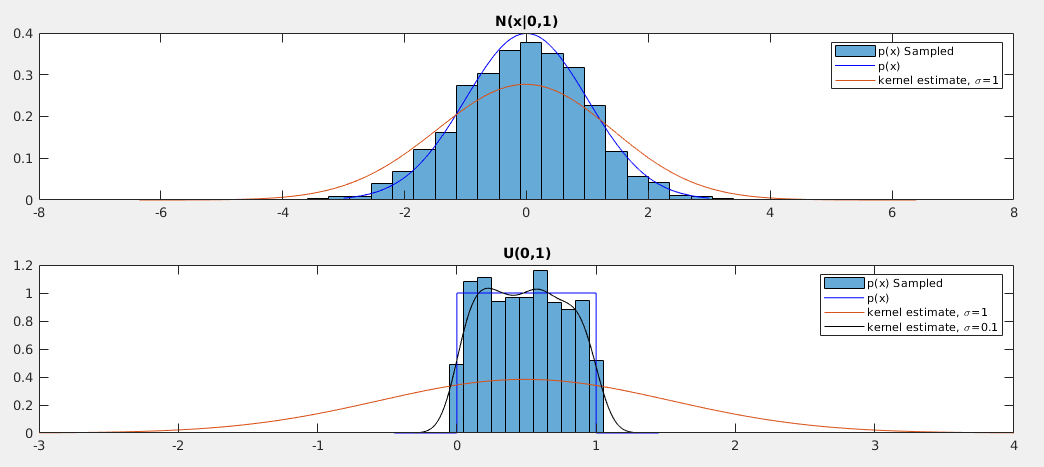
\includegraphics[width=0.9\linewidth]{task_1.png}
	\caption{Sampling and Kernel Density estimate demonstration}
	\label{fig:ksdensity}
\end{figure}


It is clearly seen, the choice of kernel size (bandwidth) determines the quality of our probability density estimate, the bandwidth of the kernel should neither be too small or too large (underfitting for larger kernels, overfitting for small kernels). The kernel density method also cannot handle discontinouties which is likely to happen on real world models. Histogram on the otherhand provides a unbiased way of visualizing the sampled distribution. However, it is difficult to perform mathematical operations on descrete data, often we need to convert it into a continous variable. The bin size of the histogram is also important, as linear bins may result in missing details for dense regions and no counts for sparse regions (this can however be resolved through entropy based binning methods).\\
Intuitively, the more number of samples we have, the more representative (accurate) the histogram is. From the theory of \textit{multinomial distribution}, we are given the mean of the count data in bin $j$ with width $\delta$ is $Np_j$ and the standard deviation is $\sqrt{Np_j(1-p_j)}$, where $p_j$ is given by:
$$
p_j = \int_{c_j-\delta/2}^{c_j+\delta/2}p(x)dx
$$
We can therefore derive that the theoretical mean count within any bins for a uniformaly distributed random variable is $N\delta$, with standard deviation $\sqrt{N\delta(1-\delta)}$. Hence the mean count varies linearly with $N$ with standard deviation only varying in square root. We are therefore expecting less variance within bins (hence more accuracy) as $N$ increases. This is confirmed through experimentation, figure \ref{fig:bins} shows how theoretical mean and standard deviation varies with $N$:
\begin{figure}[htp]
	\centering
	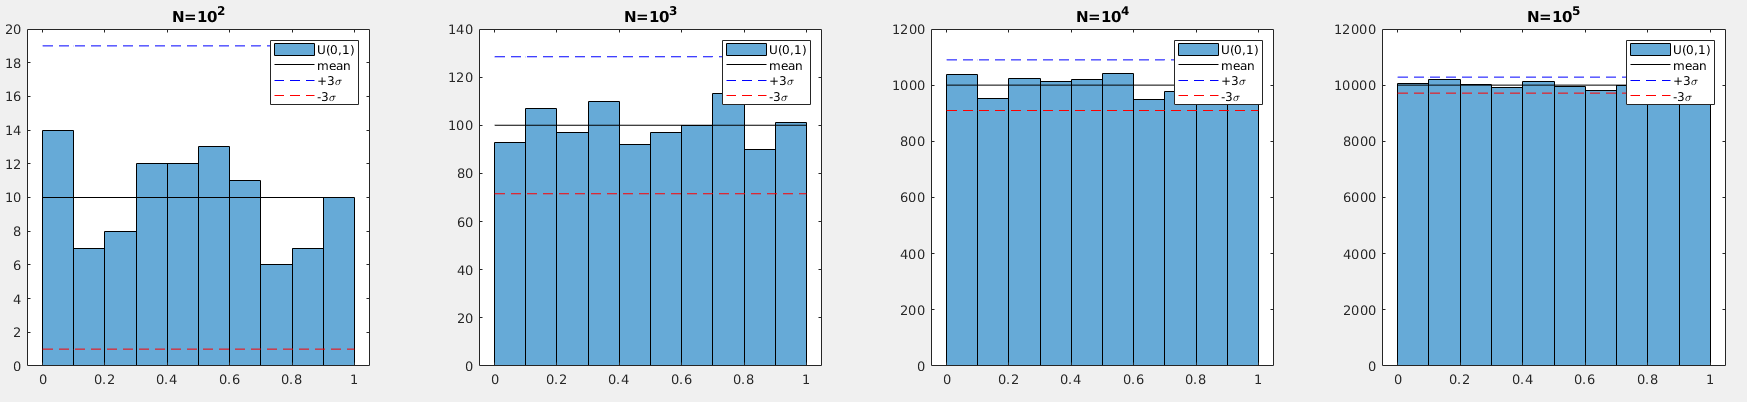
\includegraphics[width=\linewidth]{task_1_2.png}
	\caption{Sampling accuracy for uniform distribution}
	\label{fig:bins}
\end{figure}

\section{Functions of Random Variables}
\newcommand\given[1][]{\:#1\vert\:}

It is shown that given a random variable $x$, with density function $p(x)$ and there exists a function which maps $x$ to another variable so that $y=f(x)$, the density function of $p(y)$ can be found using the Jacobian method, note $x_k(y)$ denotes the possible solution for $f^{-1}(y)$, if $f(y)$ is a one-to-one mapping function, then we can ignore the summation.:
\begin{equation}
p(y) = \sum_{k=1}^{K}\dfrac{p(x)}{|dy/dx|} \given _{x=x_k(y)}
\label{eq:jacobian}
\end{equation}
Using this theorum, for normally distributed $\mathcal{N}(x|0,1)$ random variables, take $y=f(x)=ax+b$, we aim to derive the density function $p(y)$. First, we write out the full form of our input distribution:
\begin{equation}
	p(x) = \mathcal{N}(x|0,1) = \dfrac{1}{\sqrt{2\pi}}e^{-x^2/2}
\end{equation}
given $y=ax+b$, differentiating we have:
\begin{equation}
\dfrac{dy}{dx} = a \quad \forall x
\end{equation}
We also have $f^{-1}(y)=\dfrac{y-b}{a}$, subsituting these into equation \ref{eq:jacobian}, we have:
\begin{eqnarray}
	p(y)&=&\dfrac{p(x)}{a}\given x(y)=\dfrac{y-b}{a}\\
	p(y) &=& \dfrac{1}{\sqrt{2\pi a^2}}e^{-{(y-b)^2/2a^2}} = \mathcal{N}(y|b,a)
\end{eqnarray}
Therefore, we are expecting a normal distribution centred around $b$ with a standard deviation of $a$. Left Figure \ref{fig:jacobian} demonstrates exactly this if $a=2$ and $b=3$, we indeed see $p(y)$ is a normal distribution with correct mean and standard deviation.\\

\begin{figure}[htp]
	\centering
	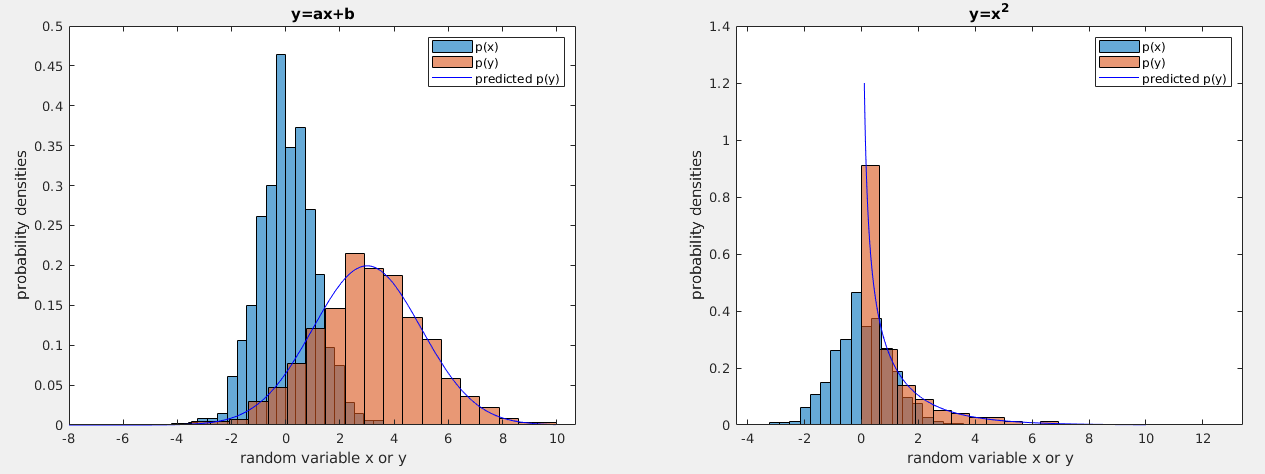
\includegraphics[width=0.9\linewidth]{task_2.png}
	\caption{Functions of random variables probability density mapping}
	\label{fig:jacobian}
\end{figure}
Similarly, if instead $y=x^2$, following the same derivation, we arrive at the probability density function below. This is also confirmed by the experimental plot shown on the right of figure \ref{fig:jacobian}:
\begin{equation}
	p(y)=\dfrac{1}{\sqrt{2\pi y}}e^{-y/2}
\end{equation}

\section{Inverse Cumulative Frequency Density Method}
Transformations of random variables leads to a very general method for non-uniform random variable generation. One of the simplest methods for generation of random variates with specified probability density is the \textit{Cumulative Frequency Density} (CFD) method. It states that for any target probability distribution $p(y)$ that has an invertable CFD denoted by $F^{-1}(x)$, we can achive the target distribution $p(y)$ by transforming random variables sampled from a uniform distribution $p(x)=\mathcal{U}(0,1)$ through:
\begin{equation}
	y = f(x) = F^{-1}(x)
\end{equation}
For example, given a target exponential distribution $p(y) = \exp(-y)$ we first compute its CFD and Inverse CFD, $F(X)$ and $F^{-1}(x)$ respectively:
\begin{eqnarray}
	F(X)=\int_{0}^{X}p(y)=1-e^{-X}\\
	F^{-1}(X')=-\ln (1-X')
\end{eqnarray}
Using the equation above, random variables sampled from a uniform distribution $p(x)=U(0,1)$ is passed through the mapping function $F^{-1}(x)$, figure \ref{fig:cdf} shows histograms and kernel density estimates of this transformation with actual target ditribution overlayed on top. We can see clearly that the inverse CFD method can be used to generate reliable samples.
\begin{figure}[htp]
 \centering
 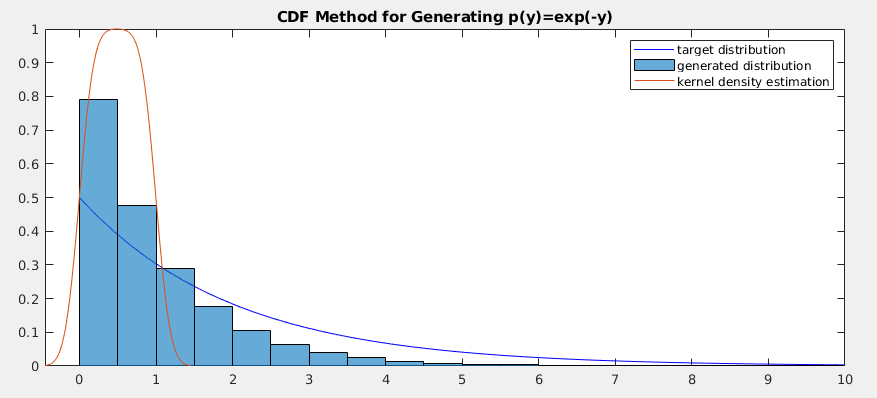
\includegraphics[width=0.7\linewidth]{task_4.png}
 \caption{Sampling accuracy for uniform distribution}
 \label{fig:cdf}
\end{figure}

\section{Stable Distribution Simulation}
Sometimes random variables cannot be simulated using inverse CDF or other convenient means. One such case is the stable distribution which is fundimental in the field of communications data, sigal processing and Internet of Things where interfering noise can be far from the Gaussian assumptions imposed.\\
There are two parameters controlling the distribution, $\alpha \in (0,2)\;\; (\alpha \neq 1)$ and $\beta \in [-1,+1]$. The distribution is drawn from two standard random variables, a uniform distribution: $U\sim \mathcal{U}(-\pi/2,+\pi/2)$ and a exponential distribution: $V\sim \mathcal{E}(V|1)$. The formula for the alpha stable distribution is quiet complex and is ommited here. Figure \ref{fig:stable} depicts the effects of parameters $\alpha$ and $\beta$ on the distribution. It is seen that the $\alpha$ parameter controls the sharpness of the rolloff of the distribution. The higher it is the more it seems to have a gaussian like behaviour (less skewed towards center). The parameter $\beta$ controls the left/right skewness of the distribution, with $-1$ meaning mean shifting more towards right, and $+1$ meaning mean shifting more towars the left.
\begin{figure}[htp]
 \centering
 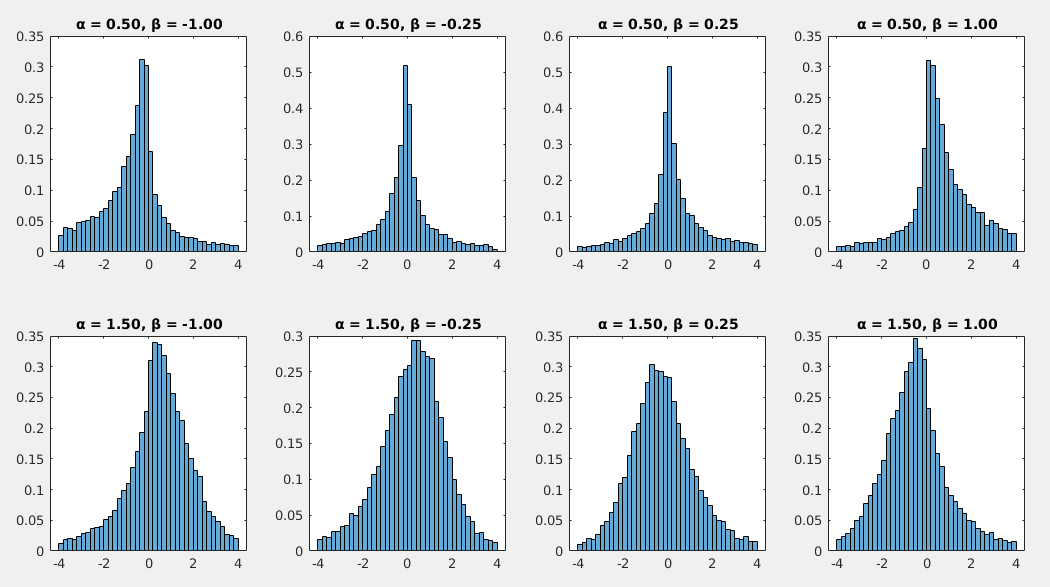
\includegraphics[width=0.9\linewidth]{task_6.png}
 \caption{Effects of parameters on Alpha-Stable Distribution}
 \label{fig:stable}
\end{figure}

\end{document}
